\chapter{Resultados y discusión} \label{chap:resultados}
% Interpretar los resultados de cómo y por qué
% - ¿Por qué el modo híbrido funciona mejor que los otros?
% - La tendencia de los pesos a irse a 0 o 1
% - Limitaciones del enfoque: bot sin memoria ni planificación, etc

Este capítulo se dedica al análisis e interpretación de los resultados obtenidos durante los experimentos detallados en el capítulo \ref{chap:experimentacion}. El objetivo no es solo presentar los datos de rendimiento de forma cuantitativa, sino también ofrecer una discusión crítica sobre por qué ciertas estrategias de entrenamiento han demostrado ser más efectivas que otras. Se intentará interpretar los valores de los pesos obtenidos en los mejores individuos de los experimentos, como la tendencia a la especialización, y se discutirán las limitaciones inherentes al algoritmo del agente. Finalmente, se concluirá el capítulo resumiendo cómo estos resultados satisfacen los objetivos finales de la investigación.

\section{Análisis de las configuraciones híbridas} \label{sec:analisis_configuraciones_hibridas}
% Unlike AlphaZero, AlphaStar initially learns to imitate the moves of the best players in its database of human vs. human games; this step is necessary to solve what DeepMind's Dave Silver calls "the exploration problem": discovering new strategies would otherwise be like finding a "needle in a haystack". Agents then play each other and deploy deep reinforcement learning. These main agents also learn by playing against suboptimal "exploiter agents" whose purpose is to expose weaknesses in the main agents (Artículo BBC). \cite{leo_kelion_deepmind_2019}
% Cuando vaya a comparar resultados, hablar del problema que tuve con 100 partidas vs 5000 partidas.

El primer bloque de experimentos se centró en evaluar el rendimiento de las 20 distintas planificaciones de entrenamiento en modo híbrido, detalladas previamente en la Tabla \ref{tab:hybrid_schedules}. Debido a las limitaciones de tiempo, se ejecutó una selección representativa de 10 de estas configuraciones. Para cada configuración, el mejor campeón obtenido tras el proceso de entrenamiento fue sometido a una rigurosa fase de validación cruzada, consistente en 20,000 partidas contra un conjunto de cuatro bots de referencia con estrategias diversas.

La Tabla \ref{tab:resultados_hibridos} resume los resultados de esta validación. La tabla está ordenada de mayor a menor según la tasa de victorias global, permitiendo identificar rápidamente las configuraciones más exitosas. Además del rendimiento general, se desglosa la tasa de victorias contra cada uno de los cuatro oponentes estáticos, lo que permite analizar si ciertas planificaciones tienden a generar agentes especialistas o generalistas.

\begin{table}[H]
	\centering
	\caption{Rendimiento de los campeones generados por 10 configuraciones del modo híbrido, ordenados por su tasa de victorias global.}
	\label{tab:resultados_hibridos}
	\begin{tabular}{@{}lccccc@{}}
		\toprule
		\textbf{ID} & \textbf{Tasa Vict.} & \textbf{vs Patron} & \textbf{vs Agents} & \textbf{vs Prestige} & \textbf{vs Tree} \\
		\midrule
		H-3                 & 48.20\%                   & 70.0\%                & 65.3\%                & 34.3\%                  & 23.3\%              \\
		H-1                 & 46.31\%                   & 69.1\%                & 68.1\%                & 27.8\%                  & 20.3\%              \\
		H-5                 & 43.73\%                   & 58.4\%                & 54.1\%                & 38.2\%                  & 24.1\%              \\
		H-6                 & 34.70\%                   & 42.9\%                & 20.1\%                & 53.2\%                  & 22.6\%              \\
		H-4                 & 34.49\%                   & 43.0\%                & 18.9\%                & 51.8\%                  & 24.3\%              \\
		H-8                 & 34.16\%                   & 54.3\%                & 48.4\%                & 12.1\%                  & 21.8\%              \\
		H-7                 & 33.41\%                   & 44.9\%                & 20.5\%                & 51.4\%                  & 16.8\%              \\
		H-10                & 33.25\%                   & 43.6\%                & 20.9\%                & 52.3\%                  & 16.1\%              \\
		H-2                 & 32.62\%                   & 42.7\%                & 20.3\%                & 52.2\%                  & 15.3\%              \\
		H-9                 & 31.85\%                   & 32.3\%                & 63.1\%                & 12.4\%                  & 19.7\%              \\
		\bottomrule
	\end{tabular}
\end{table}

\begin{figure}[H]
	\centering
	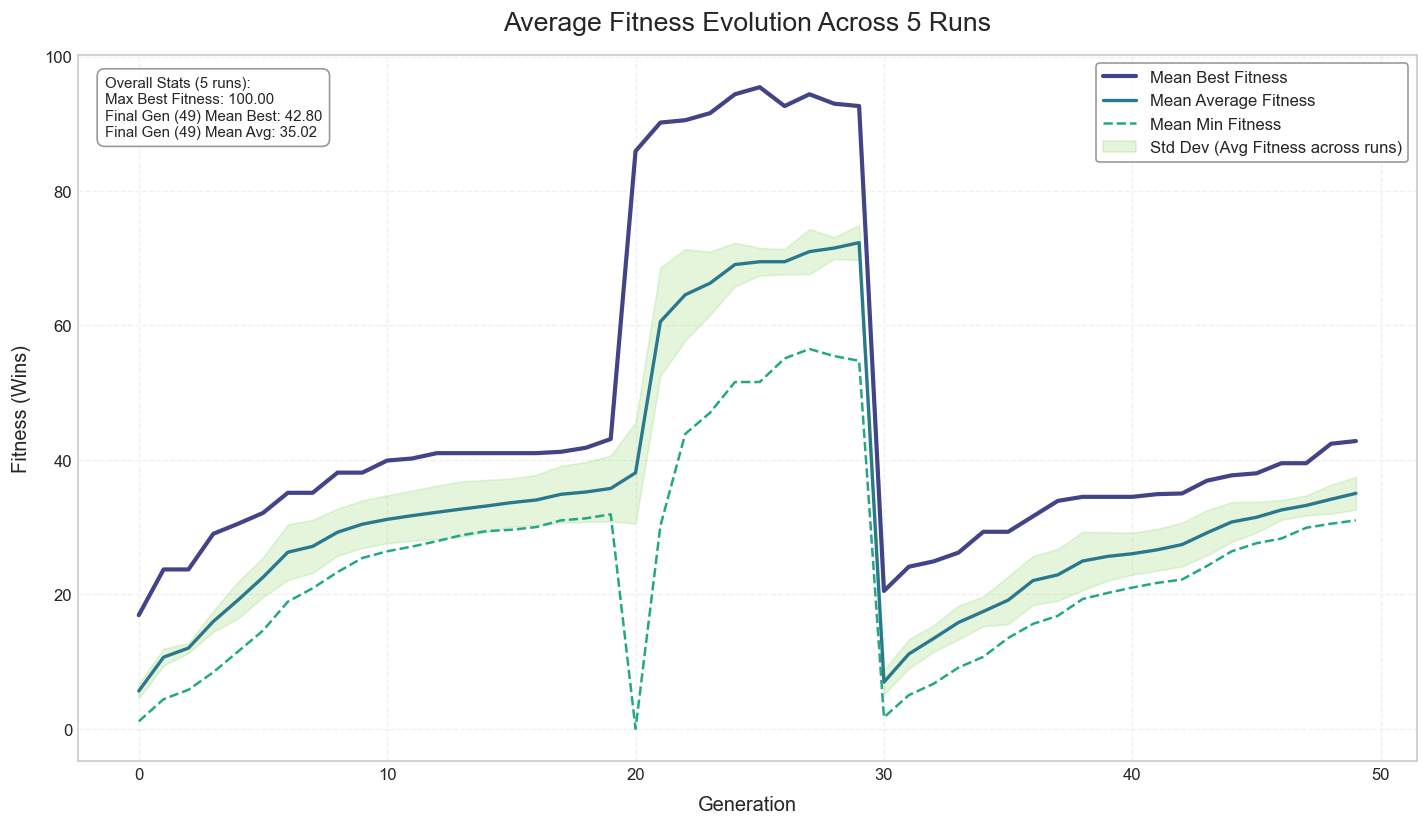
\includegraphics[width=1.0\textwidth]{img/fitness_evolution_424.png}
	\caption{Evolución del fitness sobre las generaciones para la combinación híbrida ganadora.}
	\label{fig:fitness_evolution_424}
\end{figure}

\section{Análisis de los modos de entrenamiento} \label{sec:analisis_modos_entrenamiento}


\section{Análisis del salón de la fama} \label{sec:analisis_salon_fama}




% Decir que se han cumplido los dos objetivos faltantes:
% OG5: Evaluar cuantitativamente el rendimiento del agente entrenado mediante las diferentes estrategias, utilizando métricas relevantes.
% OG6: Analizar comparativamente la efectividad y eficiencia de las estrategias de optimización implementadas, discutiendo sus ventajas y desventajas en el contexto específico de ``Scripts of Tribute''.
% Decir que así concluye el cumplimiento de todos los objetivos específicos del proyecto.



